%\hypertarget{___gatsby}{}
%\hypertarget{gatsby-focus-wrapper}{}
%\href{https://mukulrathi.com/}{}
%
%MUKUL RATHI
%
%\href{https://mukulrathi.com/about-me}{}
%
%About Me
%
%\href{https://mukulrathi.com/blog}{}
%
%Blog
%
%\hypertarget{creating-the-bolt-compiler-part-2}{%
%\subsection{Creating the Bolt Compiler: Part
%2}\label{creating-the-bolt-compiler-part-2}}

\hypertarget{top-of-page}{%
\chapter{So how do you structure a compiler
project?}\label{top-of-page}}

%\hypertarget{may-25-2020}{%
%\subsection{May 25, 2020}\label{may-25-2020}}

May 25, 2020

%\hypertarget{min-read}{%
%\subsection{6 min read}\label{min-read}}
%
%\hypertarget{last-updated-january-10-2021}{%
%\subsection{Last updated: January 10,
%2021}\label{last-updated-january-10-2021}}

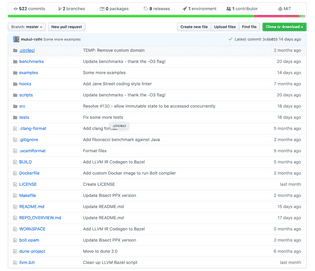
\includegraphics[width=\linewidth]{02_files/repo-overview.png}

%\hypertarget{series-creating-the-bolt-compiler}{%
%\section{Series: Creating the Bolt
%Compiler}\label{series-creating-the-bolt-compiler}}

%\begin{itemize}
%\item
%  { Part 1:
%  }\href{https://mukulrathi.com/create-your-own-programming-language/intro-to-compiler/}{How
%  I wrote my own "proper" programming language}
%\item
%  \textbf{Part 2: So how do you structure a compiler project?}
%\item
%  { Part 3:
%  }\href{https://mukulrathi.com/create-your-own-programming-language/parsing-ocamllex-menhir/}{Writing
%  a Lexer and Parser using OCamllex and Menhir}
%\item
%  { Part 4:
%  }\href{https://mukulrathi.com/create-your-own-programming-language/intro-to-type-checking/}{An
%  accessible introduction to type theory and implementing a
%  type-checker}
%\item
%  { Part 5:
%  }\href{https://mukulrathi.com/create-your-own-programming-language/data-race-dataflow-analysis/}{A
%  tutorial on liveness and alias dataflow analysis}
%\item
%  { Part 6:
%  }\href{https://mukulrathi.com/create-your-own-programming-language/lower-language-constructs-to-llvm/}{Desugaring
%  - taking our high-level language and simplifying it!}
%\item
%  { Part 7:
%  }\href{https://mukulrathi.com/create-your-own-programming-language/protobuf-ocaml-cpp-tutorial/}{A
%  Protobuf tutorial for OCaml and C++}
%\item
%  { Part 8:
%  }\href{https://mukulrathi.com/create-your-own-programming-language/llvm-ir-cpp-api-tutorial/}{A
%  Complete Guide to LLVM for Programming Language Creators}
%\item
%  { Part 9:
%  }\href{https://mukulrathi.com/create-your-own-programming-language/concurrency-runtime-language-tutorial/}{Implementing
%  Concurrency and our Runtime Library}
%\item
%  { Part 10:
%  }\href{https://mukulrathi.com/create-your-own-programming-language/generics-parametric-polymorphism/}{Generics
%  - adding polymorphism to Bolt}
%\item
%  { Part 11:
%  }\href{https://mukulrathi.com/create-your-own-programming-language/inheritance-method-overriding-vtable/}{Adding
%  Inheritance and Method Overriding to Our Language}
%\end{itemize}

\begin{center}\rule{0.5\linewidth}{0.5pt}\end{center}

Writing a compiler is like any other software engineering project in
that it involves a lot of key design decisions: what language do you
use, how do you organise your files in the repo, which tools should you
be using? Most compiler tutorials focus on a toy example and choose to
ignore these practical concerns.

With \emph{Bolt}, I'd like to highlight a larger compiler and the design
decisions I've made. If you're reading this and you work on an
industrial compiler for a more mature language,
\href{https://twitter.com/mukulrathi_}{please reach out on Twitter}! I'd
love to hear about the design decisions you took!

\hypertarget{use-the-right-language-for-the-job-not-just-the-language-you-know-best}{%
\section{\texorpdfstring{\protect\hyperlink{use-the-right-language-for-the-job-not-just-the-language-you-know-best}{}Use
the right language for the job, not just the language you know
best}{Use the right language for the job, not just the language you know best}}\label{use-the-right-language-for-the-job-not-just-the-language-you-know-best}}

\textbf{``Write a compiler using language Y''} (insert your favourite
language) tutorials are a dime a dozen. It might seem easier initially
to write a compiler using a language you know, as it's one less thing to
learn, but this is only a short-term gain. Choosing the correct language
is like learning to touch-type: sure it will be slower to start with,
but just think of how much faster you'll be once you've got to grips
with it!

JavaScript is a great language for web apps and easy to pick up for
beginners. But would I write a compiler in it? \textbf{Frankly, no.} I'm
not hating on JavaScript (I use it in this very site), it just doesn't
suit our goal.

What do we care about for compilers?

\begin{itemize}
\item
  \textbf{Coverage} - we need to consider all possible Bolt expressions
  and make sure we handle all cases - it's no good if our compiler
  crashes on Bolt programs we forgot to consider. Does our language help
  us keep track of this?
\item
  \textbf{Data representation} - how do we represent and manipulate Bolt
  expressions in the compiler?
\item
  \textbf{Tooling} - does our language have libraries we can use for our
  compiler? There's a balance between learning by doing and
  unnecessarily reinventing the wheel.
\item
  \textbf{Speed} - there are two different aspects. Firstly, how fast is
  the compiled Bolt code? Secondly, how fast is the compiler (how long
  does it take to compile the Bolt code)? There's a tradeoff - to get
  faster compiled code, you need to include more optimisation steps in
  your compiler, making the compiler slower.
\end{itemize}

There's no silver bullet: each compiler design inherently has its
tradeoffs. I chose to primarily write my compiler in OCaml.

\hypertarget{why-ocaml}{%
\section{\texorpdfstring{\protect\hyperlink{why-ocaml}{}Why
OCaml?}{Why OCaml?}}\label{why-ocaml}}

OCaml is a functional programming language with a powerful type system.
You probably have two questions: why functional programming, and what do
I mean by powerful type system?

In a large compiler, there's a lot of moving parts and keeping track of
state makes our lives harder. Functional programming is easier to reason
about: if you pass a function the same input it will always return the
same output. With functional programming we don't have to worry about
\textbf{side-effects} or state, and it lets us focus on the high-level
design.

Another alternative is to write the compiler in Rust for performance
reasons. Whilst you might have a faster compiler, I don't think the
speed justifies the additional low-level details like managing memory
that Rust requires you to track. Personally, since I'm not writing
thousands of lines of Bolt code, I'm not too concerned with how long the
Bolt compiler takes to compile programs.

\hypertarget{types-let-you-pair-program-with-the-compiler}{%
\subsection{\texorpdfstring{\protect\hyperlink{types-let-you-pair-program-with-the-compiler}{}Types
let you pair program with the
compiler}{Types let you pair program with the compiler}}\label{types-let-you-pair-program-with-the-compiler}}

If you're coming from a dynamically typed language like JS or Python,
OCaml's rich types can feel alien and may feel cumbersome. The way I
think about types in OCaml is that they give the OCaml compiler more
information about your program - the more you tell it, the more it can
help you!

Coming back to our program of coverage, what we want to say is that a
Bolt expression is \emph{either} an integer, an if-else expression, a
method call, a while loop etc. Normally to represent something like
this, you would use an \texttt{enum} and a \texttt{switch} statement. In
OCaml we bake this ``enum'' into our type system using \emph{variant
types}. We can encode the structure of each expression within the type!
For example, to access a variable you only need to know its name
\texttt{x}. To access an object's field you need to know both its name
\texttt{x} and the field you're accessing \texttt{f}. We can then
\emph{pattern-match} based on each case: think of this like a
\texttt{switch} statement on steroids!

Copy

\begin{lstlisting}[language=caml]
type identifier =| Variable of Var_name.t| ObjField of Var_name.t * Field_name.t
let do_something id = match id with| Var(x) -> ...| ObjField(x,f) -> ...
\end{lstlisting}

I haven't even mentioned the \textbf{best part}. Because we've encoded
our Bolt expression structures in a type, the OCaml compiler will check
if we've covered all cases! That's one less thing for us to track!

So OCaml takes care of coverage, and we've decided that we'll encode
Bolt expressions as variant types, so that's the data representation
sorted. OCaml also has great tooling for the lexer and parser stages of
the compiler (discussed in the next post) which ticks off another of our
criteria.

\hypertarget{targeting-performance-with-llvm}{%
\section{\texorpdfstring{\protect\hyperlink{targeting-performance-with-llvm}{}Targeting
Performance with
LLVM}{Targeting Performance with LLVM}}\label{targeting-performance-with-llvm}}

We touched upon the fact that we don't really care about the performance
of the compiler itself. However, we do want our compiled Bolt code to be
fast (\emph{it's in the name!}). As touched on in the previous post, we
don't have to reinvent the wheel. By targeting \emph{LLVM IR}, we can
hook into the C/C++ toolchain and then get our optimisations for free!

LLVM provide APIs for language authors to generate LLVM IR - the
\emph{native} API is in C++. LLVM also offers bindings in other
languages - they are identical, just replace the C++ syntax with
whichever language you're using. LLVM actually offers OCaml bindings.

\hypertarget{why-is-the-compiler-backend-written-in-c}{%
\subsection{\texorpdfstring{\protect\hyperlink{why-is-the-compiler-backend-written-in-c}{}Why
is the compiler backend written in
C++?}{Why is the compiler backend written in C++?}}\label{why-is-the-compiler-backend-written-in-c}}

A natural question you might ask is: well why didn't you write
everything in OCaml and use the LLVM OCaml bindings?

LLVM's OCaml bindings only map some of the C++ API. At the time of
implementation there was no support for implementing memory fences (a
machine instruction needed to implement locks correctly) so I was forced
to write this part of the compiler in C++. I was also experimenting with
some other fancier memory consistency instructions only present in the
native C++ API.

I want to be frank with you, the OCaml LLVM bindings will likely be
sufficient for your language and I \textbf{encourage you to use that
instead}. See, the tradeoff with the approach I took is that now we have
to pass data between the OCaml compiler \emph{frontend} and the C++
compiler \emph{backend} using
\href{https://mukulrathi.com/create-your-own-programming-language/protobuf-ocaml-cpp-tutorial/}{Protobuf}.
Yes the C++ API has more power, but it results in a more complex
compiler.

Like I said, the LLVM API is the same in OCaml and C++ (apart from
syntax), so this tutorial still applies, just skip the
\href{https://mukulrathi.com/create-your-own-programming-language/protobuf-ocaml-cpp-tutorial/}{Protobuf}
post and use the \href{https://opam.ocaml.org/packages/llvm/}{llvm OCaml
package}!

%\hypertarget{i-make-content-about-my-software-engineering-journey-curated-in-my-newsletter}{%
%\subsection{I make content about my software engineering journey,
%curated in my
%newsletter!}\label{i-make-content-about-my-software-engineering-journey-curated-in-my-newsletter}}
%
%Tips from my time at Cambridge and Facebook, and early access to
%technical tutorials on machine learning, compilers and beyond.
%
%\href{https://newsletter.mukulrathi.com/}{Check out previous issues!}
%
%Email Address
%
%By subscribing, you agree with Revue's
%\href{https://www.getrevue.co/terms}{Terms of Service} and
%\href{https://www.getrevue.co/privacy}{Privacy Policy}.

\hypertarget{software-engineering-methodology}{%
\section{\texorpdfstring{\protect\hyperlink{software-engineering-methodology}{}Software
Engineering
Methodology}{Software Engineering Methodology}}\label{software-engineering-methodology}}

The repository contains more information about how the compiler is
structured in
\href{https://github.com/mukul-rathi/bolt/blob/master/REPO_OVERVIEW.md}{REPO\_OVERVIEW.md}.
Most of these are general software engineering tips so I'll keep this
brief. (If you want more detail, feel free to reach out!)

Firstly, the repository is structured to be \emph{modular}. Each stage
of the compiler has its own library,
\href{http://mukul-rathi.github.io/bolt}{whose documentation you can
view}. Functions are grouped into \emph{modules} (the \texttt{.ml} file
provides the implementation for the module, and the \texttt{.mli} file
provides the module interface). You can think of each module as
performing a certain role within a stage e.g. \texttt{type\_expr.ml}
type-checks expressions, \texttt{pprint\_parser\_tokens.ml}
pretty-prints parser tokens. It makes each module more focused, and
avoids monolithic hundreds-of-lines-long files that are hard to read.

To build these files I use the Dune build system for OCaml (I have a
\href{https://mukulrathi.com/ocaml-tooling-dune/}{blog post explaining
it}) and the Bazel build system for C++. For large repositories,
manually compiling each file (e.g. by running \texttt{clang++\ foo.cpp})
and linking files that depend on each other is nigh on impossible -
build systems automate this for us (running one \texttt{make\ build}
command will compile all the files in the repository). One of the main
benefits of Bazel is that the dependencies are all self-contained so
will work across machines.

For testing, the main library I use is the Jane Street's \textbf{Expect
tests} library. This library is \emph{really easy} to write tests for as
it autogenerates the expected output. I have a
\href{https://mukulrathi.com/ocaml-testing-frameworks/}{blog post on
testing in OCaml} that covers this. The post also explains how I set up
Continuous Integration (where the tests are run and documentation is
generated on each commit to the repository).

I also automate common tasks using a \texttt{Makefile} and
\href{https://github.com/mukul-rathi/bolt/tree/master/scripts}{some
scripts}. One tool I would highly recommend is an autoformatter - I use
\texttt{ocamlformat} for the OCaml code and \texttt{clang-format} for
the C++ code - this formats your code for you so you have pretty looking
code for free! You can automate it with the git pre-commit hook in the
repo (which will lint and format your code every time you're about to
commit) or via IDE format-on-save integration. One final tip: use
\href{https://marketplace.visualstudio.com/items?itemName=freebroccolo.reasonml}{VSCode's
OCaml IDE extension} or the equivalent for your IDE - whenever you hover
over a function it will display its type signature and any documentation
comments associated with it.

\hypertarget{summary}{%
\section{\texorpdfstring{\protect\hyperlink{summary}{}Summary}{Summary}}\label{summary}}

In these first couple of posts, I've explained where Bolt sits in the
spectrum of programming languages, and the compiler design and software
engineering decisions made. In the next post, we'll actually get to
building this. Before we do, I have a couple of action items for you:

\begin{itemize}
\tightlist
\item
  Get up to speed with OCaml.
  \href{https://dev.realworldocaml.org/}{Real World OCaml} is a great
  free resource.
\item
  \href{https://github.com/mukul-rathi/bolt}{Fork the repo.} Have a
  quick high-level scan but don't worry about the details just yet!
  We'll break down each stage of the compiler in its own post, and
  dedicate entire posts to the more complex language features.
\end{itemize}
%
%\hypertarget{share-this-on-twitter}{%
%\subsection{Share This On Twitter}\label{share-this-on-twitter}}
%
%If you liked this post, please consider sharing it with your network. If
%you have any questions, tweet away and I'll answer :) I also tweet when
%new posts drop!
%
%\textbf{PS:} I also share helpful tips and links as I'm learning - so
%you get them \textbf{well before} they make their way into a post!
%
%\hypertarget{series-creating-the-bolt-compiler-1}{%
%\section{Series: Creating the Bolt
%Compiler}\label{series-creating-the-bolt-compiler-1}}
%
%\begin{itemize}
%\item
%  { Part 1:
%  }\href{https://mukulrathi.com/create-your-own-programming-language/intro-to-compiler/}{How
%  I wrote my own "proper" programming language}
%\item
%  \textbf{Part 2: So how do you structure a compiler project?}
%\item
%  { Part 3:
%  }\href{https://mukulrathi.com/create-your-own-programming-language/parsing-ocamllex-menhir/}{Writing
%  a Lexer and Parser using OCamllex and Menhir}
%\item
%  { Part 4:
%  }\href{https://mukulrathi.com/create-your-own-programming-language/intro-to-type-checking/}{An
%  accessible introduction to type theory and implementing a
%  type-checker}
%\item
%  { Part 5:
%  }\href{https://mukulrathi.com/create-your-own-programming-language/data-race-dataflow-analysis/}{A
%  tutorial on liveness and alias dataflow analysis}
%\item
%  { Part 6:
%  }\href{https://mukulrathi.com/create-your-own-programming-language/lower-language-constructs-to-llvm/}{Desugaring
%  - taking our high-level language and simplifying it!}
%\item
%  { Part 7:
%  }\href{https://mukulrathi.com/create-your-own-programming-language/protobuf-ocaml-cpp-tutorial/}{A
%  Protobuf tutorial for OCaml and C++}
%\item
%  { Part 8:
%  }\href{https://mukulrathi.com/create-your-own-programming-language/llvm-ir-cpp-api-tutorial/}{A
%  Complete Guide to LLVM for Programming Language Creators}
%\item
%  { Part 9:
%  }\href{https://mukulrathi.com/create-your-own-programming-language/concurrency-runtime-language-tutorial/}{Implementing
%  Concurrency and our Runtime Library}
%\item
%  { Part 10:
%  }\href{https://mukulrathi.com/create-your-own-programming-language/generics-parametric-polymorphism/}{Generics
%  - adding polymorphism to Bolt}
%\item
%  { Part 11:
%  }\href{https://mukulrathi.com/create-your-own-programming-language/inheritance-method-overriding-vtable/}{Adding
%  Inheritance and Method Overriding to Our Language}
%\end{itemize}
%
%\begin{itemize}
%\item ~
%  \hypertarget{how-i-wrote-my-own-proper-programming-language}{%
%  \subsection{\texorpdfstring{\href{https://mukulrathi.com/create-your-own-programming-language/intro-to-compiler/}{←
%  How I wrote my own "proper" programming
%  language}}{← How I wrote my own "proper" programming language}}\label{how-i-wrote-my-own-proper-programming-language}}
%\item ~
%  \hypertarget{writing-a-lexer-and-parser-using-ocamllex-and-menhir}{%
%  \subsection{\texorpdfstring{\href{https://mukulrathi.com/create-your-own-programming-language/parsing-ocamllex-menhir/}{Writing
%  a Lexer and Parser using OCamllex and Menhir
%  →}}{Writing a Lexer and Parser using OCamllex and Menhir →}}\label{writing-a-lexer-and-parser-using-ocamllex-and-menhir}}
%\end{itemize}
%
%\hypertarget{table-of-contents}{%
%\section{Table of Contents}\label{table-of-contents}}
%
%\href{https://mukulrathi.com/create-your-own-programming-language/compiler-engineering-structure/\#top-of-page}{}
%
%\hypertarget{so-how-do-you-structure-a-compiler-project}{%
%\subsection{So how do you structure a compiler
%project?}\label{so-how-do-you-structure-a-compiler-project}}
%
%\begin{itemize}
%\item
%  \href{https://mukulrathi.com/create-your-own-programming-language/compiler-engineering-structure/\#use-the-right-language-for-the-job-not-just-the-language-you-know-best}{}
%
%  \hypertarget{use-the-right-language-for-the-job-not-just-the-language-you-know-best-1}{%
%  \subsection{Use the right language for the job, not just the
%  language you know
%  best}\label{use-the-right-language-for-the-job-not-just-the-language-you-know-best-1}}
%\item
%  \href{https://mukulrathi.com/create-your-own-programming-language/compiler-engineering-structure/\#why-ocaml}{}
%
%  \hypertarget{why-ocaml-1}{%
%  \subsection{Why OCaml?}\label{why-ocaml-1}}
%
%  \begin{itemize}
%  \item
%    \href{https://mukulrathi.com/create-your-own-programming-language/compiler-engineering-structure/\#types-let-you-pair-program-with-the-compiler}{}
%
%    \hypertarget{types-let-you-pair-program-with-the-compiler-1}{%
%    \subsection{Types let you pair program with the
%    compiler}\label{types-let-you-pair-program-with-the-compiler-1}}
%  \end{itemize}
%\item
%  \href{https://mukulrathi.com/create-your-own-programming-language/compiler-engineering-structure/\#targeting-performance-with-llvm}{}
%
%  \hypertarget{targeting-performance-with-llvm-1}{%
%  \subsection{Targeting Performance with
%  LLVM}\label{targeting-performance-with-llvm-1}}
%
%  \begin{itemize}
%  \item
%    \href{https://mukulrathi.com/create-your-own-programming-language/compiler-engineering-structure/\#why-is-the-compiler-backend-written-in-c}{}
%
%    \hypertarget{why-is-the-compiler-backend-written-in-c-1}{%
%    \subsection{Why is the compiler backend written in
%    C++?}\label{why-is-the-compiler-backend-written-in-c-1}}
%  \end{itemize}
%\item
%  \href{https://mukulrathi.com/create-your-own-programming-language/compiler-engineering-structure/\#software-engineering-methodology}{}
%
%  \hypertarget{software-engineering-methodology-1}{%
%  \subsection{Software Engineering
%  Methodology}\label{software-engineering-methodology-1}}
%\item
%  \href{https://mukulrathi.com/create-your-own-programming-language/compiler-engineering-structure/\#summary}{}
%
%  \hypertarget{summary-1}{%
%  \subsection{Summary}\label{summary-1}}
%\end{itemize}
%
%© Mukul Rathi 2023
%
%\hypertarget{gatsby-announcer}{}
%Navigated to So how do you structure a compiler project?
